\chapter{Background}
\label{chap:background}

In this chapter, we provide the relevant technical background required to understand our work. We start by introducing the optimisation problem in \cref{sec:optimisation_problem}. This is continued by a mathematical formulation of the optimisation landscape in \cref{sec:optimisation_landscape}. We then discuss optimisation in deep learning in \cref{sec:optimisation_in_deep_learning}. We end this chapter with a discussion of computationally tractable methods for curvature exploitation in \cref{sec:tractable_curvature_exploitation}.

\section{The Optimisation Problem}
\label{sec:optimisation_problem}

In this section, we formalise the optimisation problem. In the most fundamental case, we minimise an objective function $f$ with respect to real-valued variables with no constraints. The formulation is 
\begin{align}
    \min_{x} f(x)
\end{align}
where
\begin{itemize}
    \item $x \in \mathbb{R}^n$ is a real-valued vector with $n \geq 1$ components,
    \item $f: \mathbb{R}^n \to \mathbb{R}$ is a real-valued function,
    \item $f \in C^k$ s.t. $k \geq 1$ is smooth.
\end{itemize}
We only have a local perspective of $f$, since it is usually expensive to evaluate. We know what $f$ evaluates to on a limited set of points $x_0, x_1, \ldots, x_k$, in which we use this information to iteratively search for an optimal point $x^*$ that minimises $f$. To do this, we must understand the landscape of $f$ and the scenarios that arise when traversing it.

\section{The Optimisation Landscape}
\label{sec:optimisation_landscape}
In this section, we introduce fundamental concepts that describe the landscape of $f$, which are needed to develop and analyse optimisation algorithms. We start by introducing the notion of critical points and how to recognise them in \cref{ssec:critical_points} and \cref{ssec:recognising_critical_points}. We then discuss convexity in \cref{ssec:convexity}. This is followed by a discussion of ill-conditioning and non-smoothness in \cref{ssec:ill_conditioning_nonsmooth}.

\subsection{Critical Points}
\label{ssec:critical_points}

When exploring the landscape of an objective function, we are interested in identifying specific points of interest that characterise its features. These are called \textit{critical points}. The most desirable of these are \textit{global optima}, in which there are \textit{global minimum} or \textit{global maximum}. An example is provided in \cref{fig:global_min_max}.

\begin{definition}[Global Minimum]
    A point $x^*$ is a \textit{global minimum} if $f(x^*) \leq f(x)$ for all $x$ in the entire domain of $f$.
\end{definition}

\begin{definition}[Global Maximum]
    A point $x^*$ is a \textit{global maximum} if $f(x^*) \geq f(x)$ for all $x$ in the entire domain of $f$.
\end{definition}

\begin{figure}[h]
    \begin{subfigure}[b]{0.48\linewidth}
        \centering
        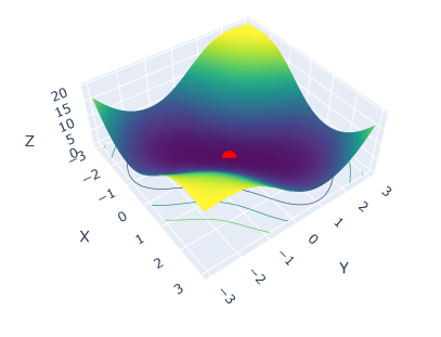
\includegraphics[width=\linewidth]{figures/2background/glob_min.png}
        \caption{A global minimum on \\
        $f(x,y) = (x-\sin(y))^2 + (y-\sin(x))^2$.}
        \label{fig:global_min}
    \end{subfigure}
    \hfill
    \begin{subfigure}[b]{0.48\linewidth}
        \centering
        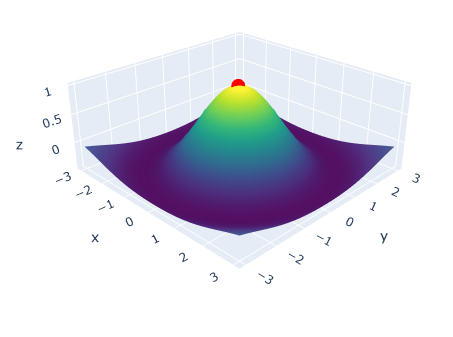
\includegraphics[width=\linewidth]{figures/2background/glob_max.png}
        \caption{A global maximum on \\
        $f(x,y) = \cos(x^2 + y^2) e^{-0.1 (x^2 + y^2)}$.}
        \label{fig:global_max}
    \end{subfigure}
    \caption{Examples of a global minimum and global maximum marked in red.}
    \label{fig:global_min_max}
\end{figure}

Finding such global optima is challenging, as we only have a limited set of information about $f$ and are resource constrained. Thus, many optimisation algorithms aim to find \textit{local optima}, which are points that are locally optimal. Similarly, there are \textit{local minimum} or \textit{local maximum}. We define these points with respect to a neighbourhood $\mathcal{N}$ of a point $x$. We provide examples in \cref{fig:local_min_max}.

\begin{definition}[Local Minimum]
    A point $x^*$ is a \textit{local minimum} if there exists a neighbourhood $\mathcal{N}$ around $x^*$ such that $f(x^*) \leq f(x)$ for all $x \in \mathcal{N}$. It is a \textit{strict local minimum} if instead $f(x^*) < f(x)$ for all $x \in \mathcal{N} \setminus \{x^*\}$.
\end{definition}

\begin{definition}[Local Maximum]
    A point $x^*$ is a \textit{local maximum} if there exists a neighbourhood $\mathcal{N}$ around $x^*$ such that $f(x^*) \geq f(x)$ for all $x \in \mathcal{N}$. It is a \textit{strict local maximum} if instead $f(x^*) > f(x)$ for all $x \in \mathcal{N} \setminus \{x^*\}$.
\end{definition}

\begin{figure}[h]
    \begin{subfigure}[b]{0.48\linewidth}
        \centering
        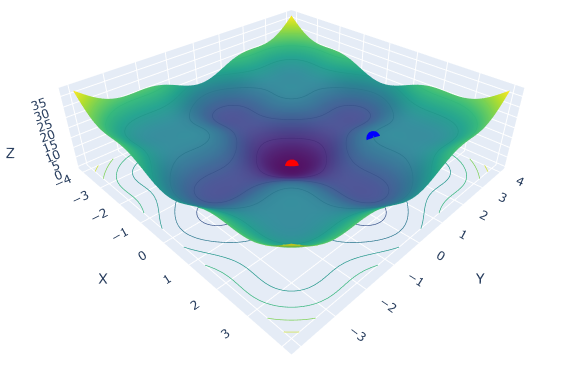
\includegraphics[width=\linewidth]{figures/2background/local_min.png}
        \caption{A local minimum on the egg crate function. \\
        $f(x,y) = (x^2 + y^2) + 5 (\sin(x)^2 + \sin(y)^2)$.
        }
        \label{fig:local_min}
    \end{subfigure}
    \hfill
    \begin{subfigure}[b]{0.48\linewidth}
        \centering
        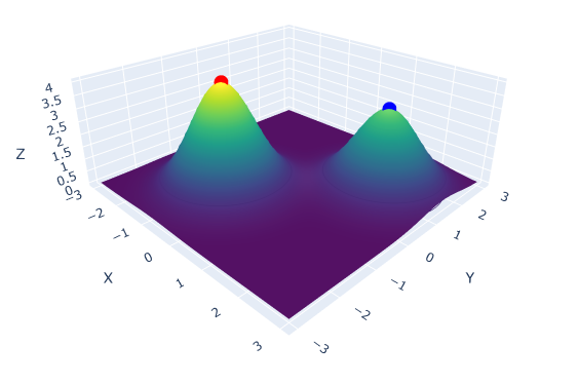
\includegraphics[width=\linewidth]{figures/2background/local_max.png}
        \caption{A local maximum on a multi-bump function. \\
        $f(x,y) = 3 e^{-(x-1.5)^2 - (y-1.5)^2} + \\
         4 e^{-(x+1)^2 - (y+1)^2} $.}
        \label{fig:local_max}
    \end{subfigure}
    \caption{Examples of a local minimum and local maximum marked in blue. The global minimum and global maximum are marked in red for comparison.}
    \label{fig:local_min_max}
\end{figure}

Beyond these, we have \textit{saddle points}. These are points that are locally flat but are neither a local minimum nor a local maximum, as seen in \cref{fig:saddle_point}. In any neighbourhood $\mathcal{N}$ around a saddle point, the function's value increases along some directions emanating from $x^*$ and decreases along others. We formally define saddle points in \cref{ssec:recognising_critical_points}.

\begin{figure}[h]
    \begin{subfigure}[b]{0.48\linewidth}
        \centering
        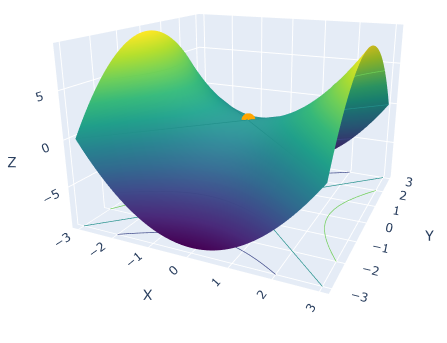
\includegraphics[width=0.8\linewidth]{figures/2background/horse_saddle.png}
        \caption{A saddle point on the horse saddle function. \\
        $f(x,y) = x^2 - y^2$.}
        \label{fig:horse_saddle}
    \end{subfigure}
    \hfill
    \begin{subfigure}[b]{0.48\linewidth}
        \centering
        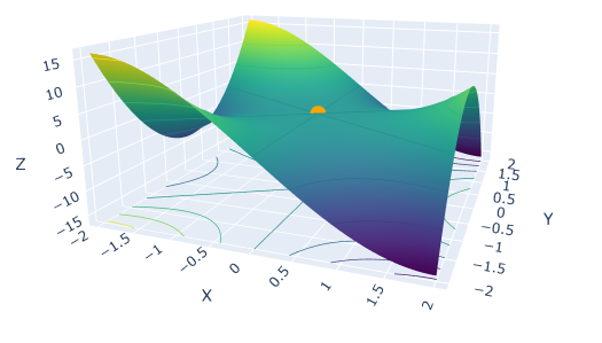
\includegraphics[width=\linewidth]{figures/2background/monkey_saddle.png}
        \caption{A saddle point on the monkey saddle function. \\
        $f(x,y) = x^3 - 3xy^2$.}
        \label{fig:monkey_saddle}
    \end{subfigure}
    \caption{Examples of two functions containing saddle points marked in orange.}
    \label{fig:saddle_point}
\end{figure}

\subsection{Recognising Critical Points}
\label{ssec:recognising_critical_points}

For smooth and differentiable functions, we can recognise critical points using the first and second order information about $f$. Here, we introduce the necessary and sufficient conditions that we use to do this. We restrict our attention to the class of functions that are twice continuously differentiable, where $f \in C^2$.

% Nit: Jacobian or gradient here?
We start with a specific type of critical point, a \textit{stationary point}. A key property of any stationary point $x^*$ is that $f$ is locally flat at $x^*$. This implies that its gradient---the vector of \textit{first-order} partial derivatives, $\nabla f(x^*)$---must be zero.
\begin{definition}[Stationary Point]
    A point $x^*$ is a \textit{stationary point} if $f$ is continuously differentiable at $x^*$ and its gradient is zero:
    \begin{align}
        \nabla f(x^*) = 0.
    \end{align}
\end{definition}

Given we are optimising $f$, we want to find a stationary point that is a local minimum. The following definition formalises the \textit{necessary first-order conditions} for a local minimum.
\begin{definition}[Necessary First-Order Conditions]
    If a point $x^*$ is a local minimum, and $f$ is continuously differentiable at $x^*$, then $\nabla f(x^*) = 0$ and $x^*$ is a stationary point.
\end{definition}

We note that all stationary points are critical points, but not all critical points are stationary points. For example, a function may have a critical point at a point where the gradient is undefined. A simple case is when $f(x) = \abs({x})$. This has a critical point at $x = 0$ where the gradient is undefined. However, given we restrict our attention to twice continuously differentiable functions, we do not need to consider these cases. 

% Nit: "Any nxn symmetric matrix A" and also specify that i < n etc.
All global optima, local optima, and saddle points are stationary points, but not all stationary points are optima. To distinguish between them, we examine the function's local curvature at $x^*$, which is captured by the \textit{Hessian matrix}---an $n \times n$ symmetric matrix of \textit{second-order} partial derivatives of $f$, denoted $\nabla^2 f(x)$ for a point $x$. We abbreviate the Hessian matrix for a function $f$ at a point $x$ as $H$ for convenience. The curvature information captured by $H$ can be summarised by its \textit{eigenvalues}. We denote the $i$-th eigenvalue of $H$, and more generally any symmetric matrix $A$, as $\lambda_i$. We use these eigenvalues to characterise two important properties, \textit{positive semidefiniteness} and \textit{negative semidefiniteness}.

\begin{definition}[Positive Semidefinite Matrix]
    An $n \times n$ symmetric matrix $A$ is \textit{positive semidefinite} if all its eigenvalues are non-negative, where $\lambda_i \geq 0$ for all $i \in [1, n]$.
\end{definition}
\begin{definition}[Negative Semidefinite Matrix]
    An $n \times n$ symmetric matrix $A$ is \textit{negative semidefinite} if all its eigenvalues are non-positive, where $\lambda_i \leq 0$ for all $i \in [1, n]$.
\end{definition}

These properties can now be used to formalise the \textit{necessary second-order conditions} to classify stationary points. We write the necessary second-order conditions for a local minimum as follows.
\begin{definition}[Necessary Second-Order Conditions]
    If a point $x^*$ is a local minimum, and $f$ is twice continuously differentiable, then:
    \begin{itemize}
        \item $\nabla f(x^*) = 0$
        \item $H$ is positive semi-definite.
    \end{itemize}
\end{definition}
Similarly, the above definition can be extended to a local maximum when $H$ is negative semi-definite.

A special case is when $H$ is \textit{indefinite}.
\begin{definition}[Indefinite Matrix]
    An $n \times n$ symmetric matrix $A$ is \textit{indefinite} if it has eigenvalues that are not all positive or negative, where $\exists \lambda_i > 0 \wedge \exists \lambda_j < 0$ for some $i, j \in [1, n]$.
\end{definition}
Here, the function curves upwards in some directions and downwards in others. This is a saddle point.

\begin{definition}[Saddle Point]
    A stationary point $x^*$ is a \textit{saddle point} if $H$ is indefinite.
\end{definition}

% Nit: Give example of strict local maximum that's guaranteed to decrease versus a flat region that's a local maximum.
Now, we can classify between local minima, local maxima, and saddle points based on whether $H$ is positive/negative semi-definite or indefinite. However, we can still fall short of distinguishing between local minima/maxima and strict local minima/maxima. For example, if $H$ is positive semidefinite, $x^*$ could be a local minimum or a flat region that is not a strict minimum. Similarly, if $H$ is negative semidefinite, $x^*$ could be a local maximum or a flat region. To distinguish between this, we consider two further properties---\textit{positive definiteness} and \textit{negative definiteness}, which are stronger conditions than positive and negative semi-definiteness.

\begin{definition}[Positive Definite Matrix]
    An $n \times n$ symmetric matrix $A$ is \textit{positive definite} if all its eigenvalues are positive, where $\lambda_i > 0$ for all $i \in [1, n]$.
\end{definition}
\begin{definition}[Negative Definite Matrix]
    An $n \times n$ symmetric matrix $A$ is \textit{negative definite} if all its eigenvalues are negative, where $\lambda_i < 0$ for all $i \in [1, n]$.
\end{definition}

We can now guarantee something stricter about the nature of $x^*$, that it is a strict local minimum/maximum. This guarantees that we will optimise our objective without being trapped in a flat region. We write these as the \textit{sufficient second-order conditions} for optimisation. We formalise this for a strict local minimum as follows.
\begin{definition}[Sufficient Second-Order Conditions]
    If $f$ is twice continuously differentiable, and $\nabla f(x^*) = 0$, and $H$ is positive definite at $x^*$, then $x^*$ is a strict local minimum.
\end{definition}
Similarly, we can write the sufficient second-order conditions for a strict local maximum when $H$ is negative definite.

We note that the sufficient second-order conditions are not necessary. A point $x^*$ may satisfy the necessary second-order conditions but fail to satisfy the sufficient second-order conditions. For example, the function $f(x) = x^4$ has a strict local minimum at $x^* = 0$, but $H$ vanishes here and is thus not positive definite at $x^*$. 

\subsection{Convexity}
\label{ssec:convexity}

The property of convexity simplifies the task of finding optima. A function $f$ is \textit{convex} if geometrically, the line segment connecting any two points on the function's graph lies on or above the graph itself. We provide an illustration in \cref{fig:convex_function}, and formally define this as follows.

% Nit: Define convex set here - potentially with a diagram.
\begin{definition}[Convex Function]
    A function $f$ is \textit{convex} if its domain is a \textit{convex set}, and for any two points $x_1, x_2$ in its domain, and any scalar $t \in [0, 1]$:
    \begin{align}
        f(t x_1 + (1-t)x_2) \leq t f(x_1) + (1-t)f(x_2).
    \end{align}
    This is a special case of \textit{Jensen's inequality}. Equivalently, a function is convex if $H$ is positive semidefinite for all $x$ in the domain of $f$ given $f$ is twice continuously differentiable.
\end{definition}

% Nit: Image resizing
\begin{figure}[h]
    \centering
    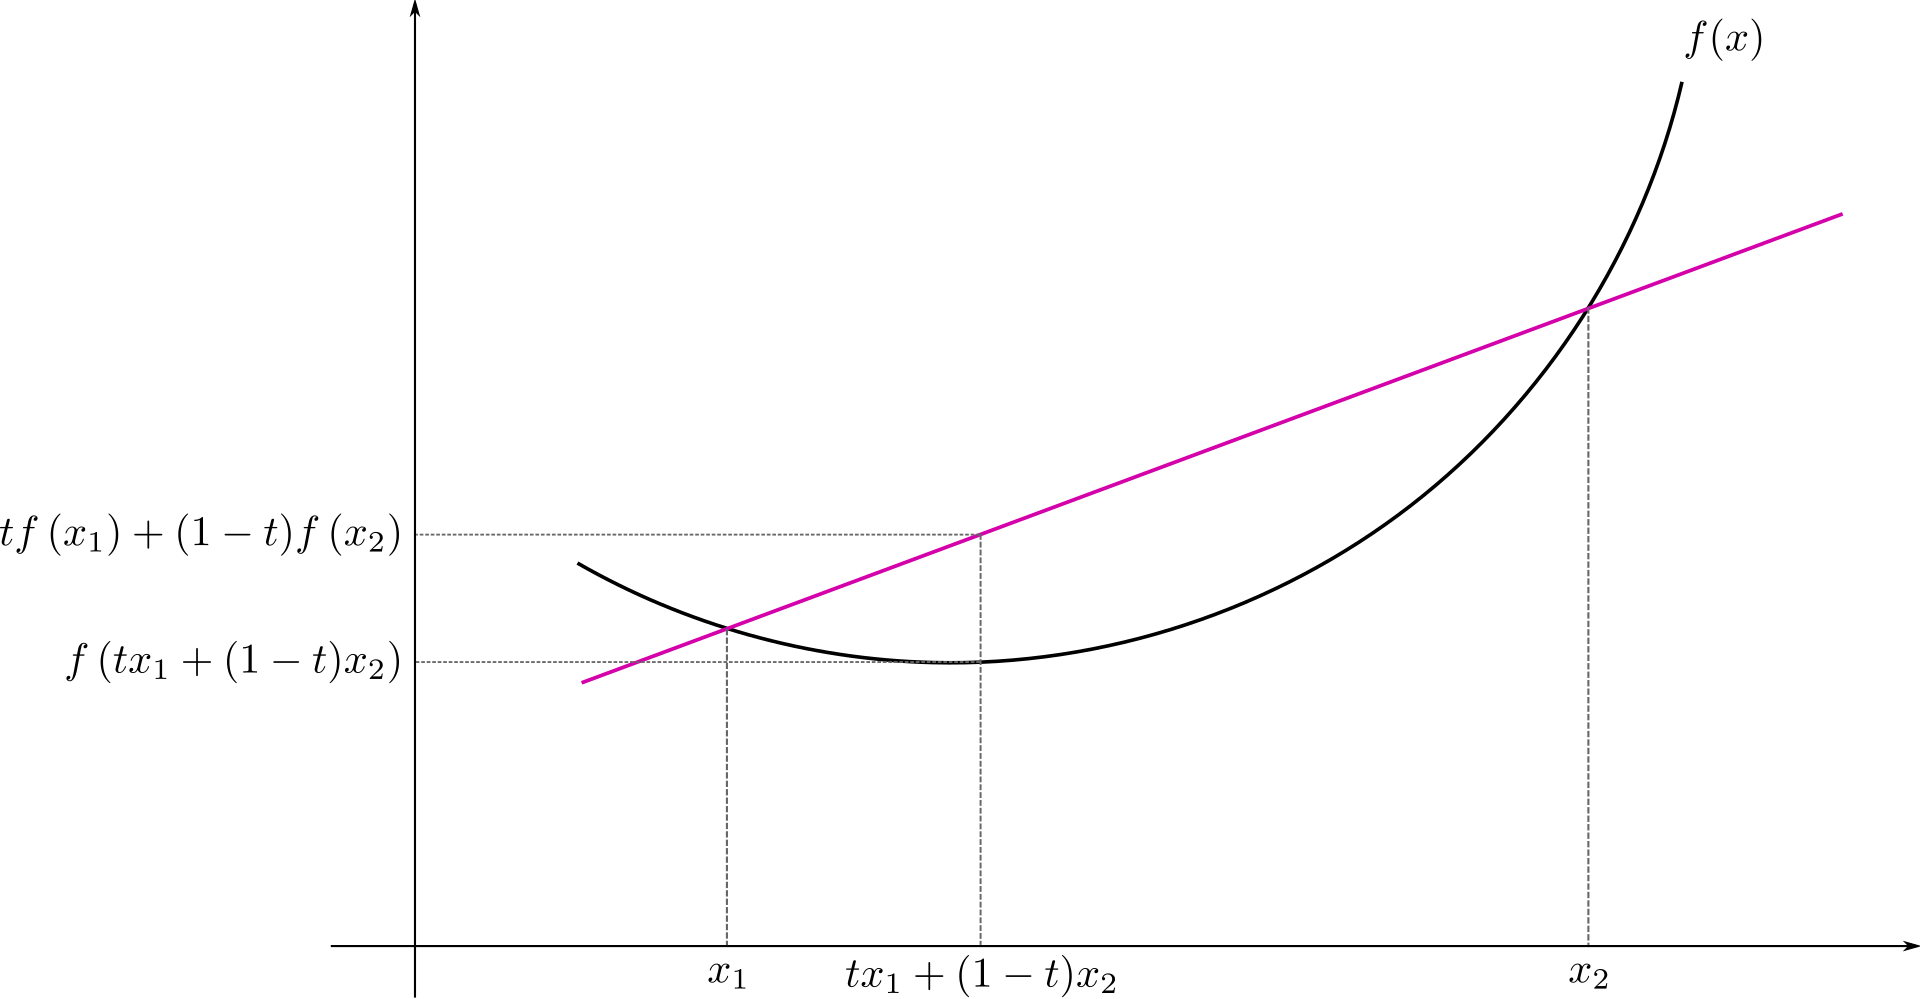
\includegraphics[width=0.7\linewidth]{figures/2background/convex_function.svg.png}
    \caption{An illustration of a convex function. The line segment created by $x_1$ and $x_2$ clearly lies above the function.}
    \label{fig:convex_function}
\end{figure}

Convex functions are particularly appealing because they possess global properties that simplify the optimisation process. We call these properties the \textit{global optimality conditions} for convex functions.

\begin{definition}[Global Optimality Conditions for Convex Functions]
    If $f$ is convex, then: 
    \begin{itemize}
        \item Any local minimum $x^*$ is a global minimum of $f$.
        \item Any stationary point $x^*$ is a global minimum of $f$ given $f$ is continuously differentiable.
    \end{itemize}
\end{definition}

This means that if we find a stationary point of a convex function, we have found the overall best possible solution. Additionally, given that $H$ is guaranteed to be positive semidefinite for twice continuously differentiable convex functions, certain optimisation algorithms can guarantee convergence to a global minimum regardless of the initialisation point. 

We can further strengthen this by considering the property of \textit{strict convexity}. A strictly convex function is one where the line segment connecting any two points on the function's graph lies strictly above the graph between those points. We illustrate the difference between convex and strictly convex functions in \cref{fig:diff_geometric_convexity}. Formally, we define strictly convex functions as follows.
\begin{definition}[Strictly Convex Function]
    A function $f: \mathbb{R}^n \to \mathbb{R}$ is \textit{strictly convex} if its domain is a convex set, and for any two distinct points $x_1, x_2$ such that $x_1 \neq x_2$ in its domain, and any scalar $t \in (0, 1)$:
    \begin{align}
        f(t x_1 + (1-t)x_2) < t f(x_1) + (1-t)f(x_2).
    \end{align}
    Equivalently, a function is strictly convex if $H$ is positive definite for all $x$ in the domain of $f$ given $f$ is twice continuously differentiable.
\end{definition}

% Nit: Make the ReLU one a bit more dark - it's hard to see the line.
\begin{figure}[h]
    \begin{subfigure}[b]{0.48\linewidth}
        \centering
        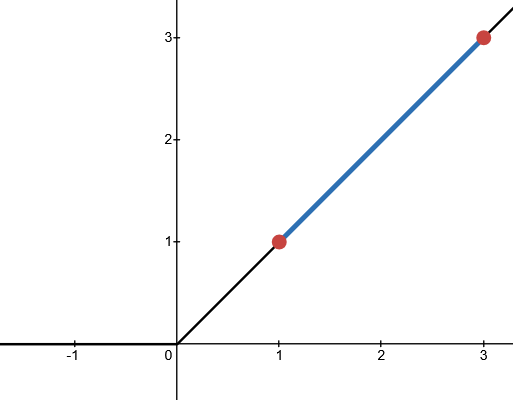
\includegraphics[width=0.8\linewidth]{figures/2background/relu.png}
        \caption{The Rectified Linear Unit (ReLU) function, $f(x) = \max(0, x)$, is convex, but not strictly convex since we can pick two points where the line segment is not strictly above the function.}
        \label{fig:convex_relu}
    \end{subfigure}
    \hfill
    \begin{subfigure}[b]{0.48\linewidth}
        \centering
        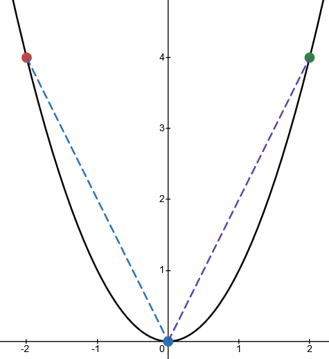
\includegraphics[width=0.6\linewidth]{figures/2background/parabola.png}
        \caption{The parabola function, $f(x) = x^2$, is strictly convex since for any two points, the line segment will always lie above the function.}
        \label{fig:strict_convex_parabola}
    \end{subfigure}
    \caption{The geometrical difference between a convex function and a strictly convex function.}
    \label{fig:diff_geometric_convexity}
\end{figure}

Strictly convex functions are a subset of convex functions. They inherit the same global optimality conditions, but with an additional \textit{uniqueness} property that makes them incredibly easy to optimise.
\begin{definition}[Uniqueness of Global Minimum]
    If $f$ is strictly convex, then there exists \textit{at most one} local minimum of $f$. Consequently, if it exists, then it is the global minimum of $f$.
\end{definition}
Thus, if we find any stationary point of a strictly convex function, we have found the global minimum. This is different from convex functions, where there could be multiple global minima. We provide an illustration of this in \cref{fig:diff_convex_functions}. This makes strictly convex functions extremely desirable for optimisation, since we have a guaranteed unique solution.

\begin{figure}[h]
    \begin{subfigure}[b]{0.48\linewidth}
        \centering
        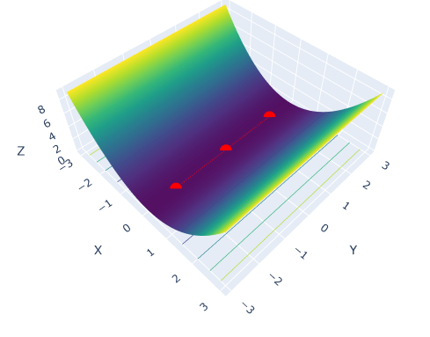
\includegraphics[width=0.8\linewidth]{figures/2background/convex_func.png}
        \caption{Multiple global minima on the convex function
        $f(x,y) = x^2$.}
        \label{fig:convex_func}
    \end{subfigure}
    \hfill
    \begin{subfigure}[b]{0.48\linewidth}
        \centering
        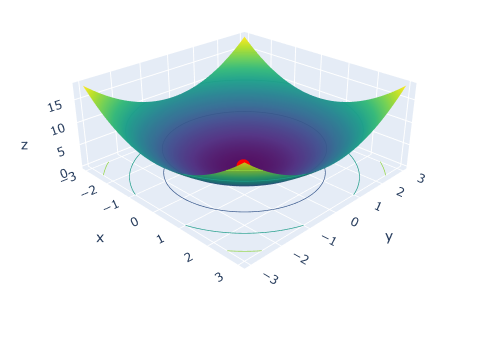
\includegraphics[width=\linewidth]{figures/2background/strict_convex.png}
        \caption{A unique global minimum on the strictly convex function
        $f(x,y) = x^2 + y^2$.}
        \label{fig:strict_convex_func}
    \end{subfigure}
    \caption{The difference between a convex function with multiple global minima and a strictly convex function with a unique global minimum.}
    \label{fig:diff_convex_functions}
\end{figure}


\subsection{Non-Smoothness and Ill-Conditioning}
\label{ssec:ill_conditioning_nonsmooth}

While convexity simplifies the process of optimisation, two other characteristics, \textit{ill-conditioning} and \textit{non-smoothness}, significantly increase the difficulty instead. We now discuss these and their influence on optimisation.

% Nit:
% - We introduce condition number based on H that is strictly convex for f, but then go on to use the Rosenbrock to demonstrate ill-conditioning with the perturbations. [FIXED]
% - We also don't show how H influences the perturbations for this, but just show an example.
% TODO - Reference the second-order methods which tackle this.
\subsubsection{Ill-Conditioning}
\label{sssec:ill_conditioning}

An optimisation problem is \textit{ill-conditioned} if the objective function $f$ is highly sensitive to small changes to its parameters in the vicinity of a solution $x^*$. Geometrically, this corresponds to a landscape that is either elongated with narrow valleys, or steep ridges with large dropoffs, as illustrated in \cref{fig:ill_conditioned_functions}. To motivate the problem of ill-conditioning, we consider the deterministic Rosenbrock function
\begin{align}
    f(x,y) = (1 - x)^2 + 100(y - x^2)^2.
    \label{eq:rosenbrock_function}
\end{align}
The global minimum for this function is at $(x,y) = (1,1)$. Suppose we introduce a small perturbation $\epsilon_1 = 0.01$ to $x$ and $\epsilon_2 = 0.02$ to $y$ around the minimum. Our function evaluates to
\begin{align}
    f(x + \epsilon_1, y + \epsilon_2) = f(1 + 0.01, 1 + 0.02)
    \approx 1e-4.
\end{align}
If we modify the perturbations to $\epsilon_1 = 0.02$ and $\epsilon_2 = -0.01$ instead, our function value now becomes
\begin{align}
    f(x + \epsilon_1, y + \epsilon_2) = f(1 + 0.02, 1 - 0.01)
    \approx 0.25.
\end{align}

\begin{figure}[h]
    \begin{subfigure}[b]{0.48\linewidth}
        \centering
        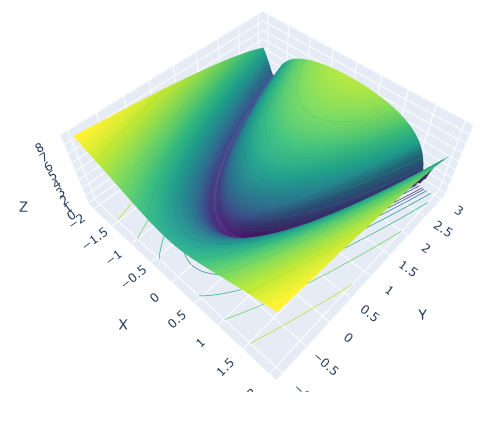
\includegraphics[width=\linewidth]{figures/2background/rosenbrock.png}
        \caption{The deterministic Rosenbrock function \\ 
        $f(x,y) = (1-x)^2 + 100(y-x^2)^2$}
        \label{fig:rosenbrock}
    \end{subfigure}
    \hfill
    \begin{subfigure}[b]{0.48\linewidth}
        \centering
        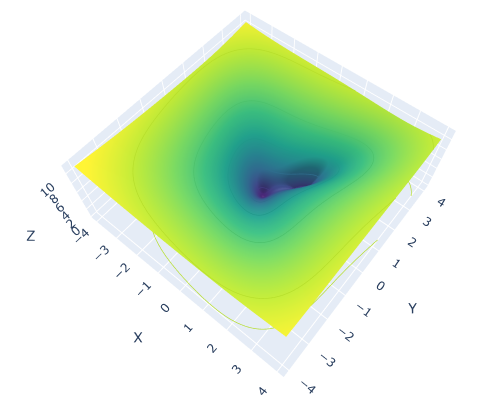
\includegraphics[width=\linewidth]{figures/2background/wood_func.png}
        \caption{A simplified 2D analogue of the wood function \\
        $f(x,y) = 100*(y - x^2)^2 + (1 - x)^2 + 90*(y^2 - x)^2 + (1 - y)^2$}
        \label{fig:wood_function}
    \end{subfigure}
    \caption{The optimisation landscape of two ill-conditioned functions. The Rosenbrock function (left) shows the narrow valley towards the minimum, whereas the 2D wood function (right) shows a steep dropoff as we approach the minimum.}
    \label{fig:ill_conditioned_functions}
\end{figure}

We see a significant change in how our function behaves, where it is now $2500$ times larger than before with only small changes applied to its input. This illustrates the problem of ill-conditioning, which makes it difficult for optimisation algorithms to converge to a solution. We describe the ill-conditioning of a problem in terms of the \textit{condition number}.

% Nit: Be consistent with the notation when you previously defined the eigenvalues before.
\begin{definition}[Condition Number]
    For any non-singular matrix $A \in \mathbb{R}^{n \times n}$, its \textit{condition number} with respect to a given matrix norm $||\cdot||$ is defined as:
    \begin{align}
        \kappa(A) = ||A||\cdot||A^{-1}||,
    \end{align}
    In the context of optimisation, if $f$ is twice continuously differentiable at $x$ and $H$ is positive definite at $x$, then the condition number is the ratio of the largest eigenvalue $\lambda_{\max}$ to the smallest eigenvalue $\lambda_{\min}$ of $H$ at $x$. 
    \begin{align}
        \kappa(H) = ||H||_2||H^{-1}||_2 = \lambda_{\max}(H)\lambda_{\max}(H^{-1}) = \lambda_{\max}(H) \cdot \frac{1}{\lambda_{\min}(H)} = \frac{\lambda_{\max}(H)}{\lambda_{\min}(H)}.
    \end{align}
\end{definition}

In the Rosenbrock example, the condition number is $2508$ at the minimum, which explains the behaviour we observed. Ill-conditioning poses significant challenges for many optimisation algorithms, especially those relying on gradient information. In these landscapes, finding solutions that are robust to perturbations is difficult. Algorithms may get stuck and make excessively small steps to counteract the ill-conditioning, which slows convergence, or they become unstable due to taking overly aggressive steps. Efficient navigation of these landscapes require algorithms to be \textit{scale invariant}. We discuss these algorithms in more detail in \cref{sec:optimisation_in_deep_learning}.

\subsubsection{Non-Smooth Problems}
\label{sssec:non_smooth_problems}

So far, we have talked about optimisation problems where the objective function $f$ is smooth and usually twice continuously differentiable. However, many optimisation problems that we encounter, particularly in machine learning, involve \textit{non-smooth functions}. These are functions that possess points at which the function or its derivatives are not well-defined. We provide an example of such functions which have points of non-differentiability in \cref{fig:non_smooth_functions}. 

\begin{figure}[h]
    \begin{subfigure}[b]{0.48\linewidth}
        \centering
        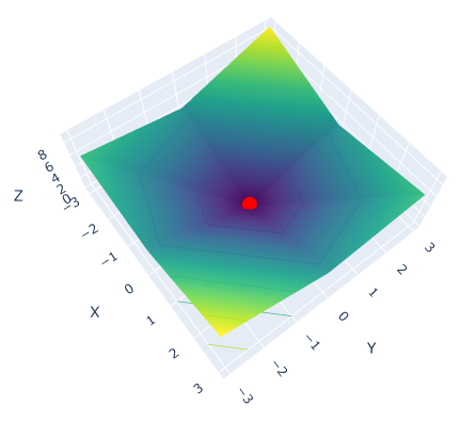
\includegraphics[width=\linewidth]{figures/2background/abs_func.png}
        \caption{The function
        $f(x, y) = |x| + |y|$ has an undefined gradient at (0,0).}
        \label{fig:abs_function}
    \end{subfigure}
    \hfill
    \begin{subfigure}[b]{0.48\linewidth}
        \centering
        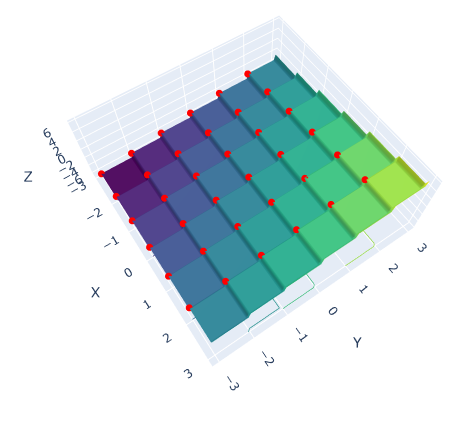
\includegraphics[width=\linewidth]{figures/2background/floor_func.png}
        \caption{The step function
        $f(x,y) = \lfloor x \rfloor + \lfloor y \rfloor$ has undefined gradients at all integer points.}
        \label{fig:step_function}
    \end{subfigure}
    \caption{The optimisation landscape of two non-smooth functions, with points of non-differentiability highlighted in red.}
    \label{fig:non_smooth_functions}
\end{figure}

Non-smoothness is common in machine learning, with terms such as ReLU and L1 regularisation being used in many problem settings. At points of non-differentiability, classical optimisation concepts that we have been discussing break down. The optimisation of non-smooth functions requires alternative theoretical frameworks and algorithms. Prominent among these are subgradient methods, which extend the concept of a gradient to non-smooth convex functions by defining a set of subgradients at each point. Bundle methods are also popular, which collect information about previous function values and subgradients to form a more sophisticated model of the objective function. We provide a more detailed overview of such methods in \cref{sec:optimisation_in_deep_learning}. In specific instances, we can reformulate the non-smooth problem into a smooth approximation. For example, the ReLU function has an equivalent smooth approximation given by the Softplus function, $f(x) = \log(1 + e^x)$.

% Nit: I don't think this is relevant it's just showing both activation functions.
% \begin{figure}[h]
%     \centering
%     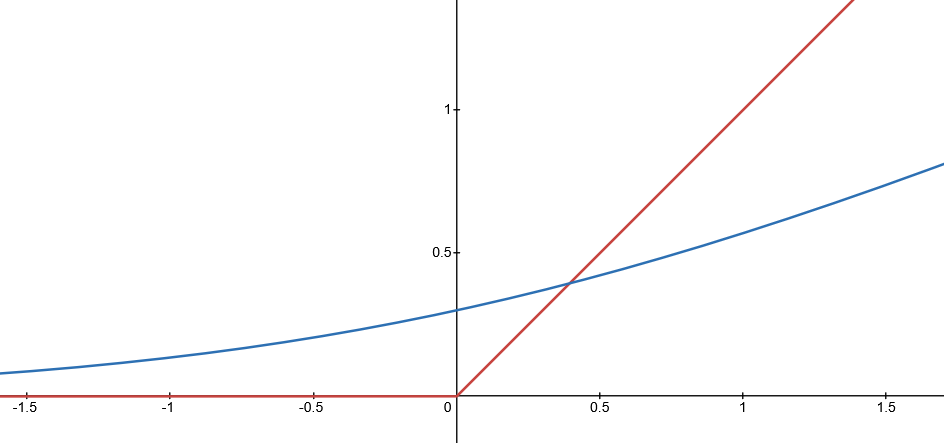
\includegraphics[width=0.8\linewidth]{figures/2background/relu_softplus.png}
%     \caption{The ReLU function (red) and its smooth approximation, the Softplus function (blue), given by $f(x) = \log(1 + e^x)$. The ReLU function is non-differentiable at $x = 0$, but the Softplus function is differentiable everywhere.}
%     \label{fig:relu_softplus}
% \end{figure} 

\section{Optimisation in Deep Learning}
\label{sec:optimisation_in_deep_learning}

% Nit: Is this actually necessary to include? I'm not sure if we'll use this notation in the thesis? [FIXED: I think this is good to have.]
Deep learning introduces a new set of challenges to the optimisation landscape. In deep learning, we usually have a set of \textit{input data} $x \in \mathbb{R}^n$ and a \textit{target output} $y \in \mathbb{R}^m$. Our goal is to learn a mapping from $x$ to $y$. This is represented by a \textit{model}, which is a complex, highly parameterised function that is usually non-convex and can be thought of as a \textit{universal function approximator}. Through exposure to many examples in a \textit{training set}, the model makes \textit{predictions} $\hat{y}$ for inputs $x$, and is then evaluated on a \textit{test set} with new, unseen inputs. Ideally, we would like our model to make accurate predictions on the test set, as this is a good indicator of generalisation performance. We optimise the model's \textit{parameters}, $\theta \in \mathbb{R}^n$, by minimising a real-valued \textit{loss function} $L: \mathbb{R}^n \to \mathbb{R}$ that measures model's performance. Typically, this is written as an average over the training set, such as
\begin{align}
    L(\theta) = \mathbb{E}_{(x, y) \sim \hat{p}_{data}} \mathcal{L}(f(x; \theta), y) = \mathbb{E}_{(x, y) \sim \hat{p}_{data}} \ell(\hat{y}, y),
\end{align}
where $\hat{y} = f(x; \theta)$, $\mathcal{L}$ is the per-example loss (such as mean-squared error or cross-entropy), and $\hat{p}_{data}$ is the empirical distribution of our training set. We limit our discussion of $\mathcal{L}$ to the \textit{supervised} learning case, where we have a fixed input $x$ and a corresponding target output $y$ and the inputs to $\mathcal{L}$ are $\hat{y}$ and $y$. It is easy to extend this development to the \textit{regularised} case, for example by including $\theta$ as an argument, or the \textit{unsupervised} case by removing $y$. 

In this section, we discuss the challenges of optimisation in deep learning. We start by discussing the behaviour of high-dimensional landscapes in \cref{ssec:dl_challenges}. This is followed by a discussion of first-order methods in \cref{ssec:first_order_methods} and second-order methods in \cref{ssec:second_order_methods}. 

\subsection{Challenges in High-Dimensional Landscapes}
\label{ssec:dl_challenges}

% TODO: Needs more rigorous citing - see 8.2 of the deep learning book and copy those references.
% TODO: Add figure about critical points + distribution graph for some dims.
High-dimensional landscapes are complex and difficult to navigate. The geometric intuition derived from low-dimensional spaces is usually not applicable. We observe two key properties in high-dimensions.
\begin{itemize}
    \item \textit{Proliferation of saddle points}: Saddle points are \textit{exponentially} more likely than local minima as dimensionality $N$ increases \citep{dauphin2014sfn}.
    \item \textit{Local minima are close to global minimum}: Local minima in high dimensions are likely to have values very close to the global minimum \citep{dauphin2014sfn,choromanska2015loss}.
\end{itemize}

% TODO: Needs ref here for the Wigner bit.
We can understand the first property by analysing $H$ in the context of our loss function, where we now have that $H = \nabla^2 L(\theta)$. As established in \cref{ssec:recognising_critical_points}, a local minimum requires all $H$ to be positive semidefinite, in which all eigenvalues are greater than or equal to zero. A saddle point however possesses both positive and negative eigenvalues. We note that for large random Gaussian matrices, the eigenvalue distribution follows \textit{Wigner's semicircle law}, which states that as $N$ increases, we observe the following.
\begin{itemize}
    \item An eigenvalue $\lambda_i$ has an equal probability of $\frac{1}{2}$ to be positive or negative. 
    \item Each eigenvalue's probability is approximately independent of others.
\end{itemize}

% TODO: Forward ref this analysis. Need ref for the second last sentence. Also need the forward ref for the last sentence.
Intuitively, we can consider the probability of each eigenvalue as akin to an independent fair coin toss. The probability of obtaining $N$ non-negative eigenvalues diminishes exponentially with increasing $N$. The same goes for obtaining $N$ non-positive eigenvalues. Consequently, obtaining $N$ eigenvalues with mixed signs are far more probable, which explains the proliferation of saddle points. While we have this case for large random Gaussian matrices, we note that this applies to the deep learning setting as well. Experimental evidence shows that the landscapes of deep learning models display many more saddle points than local minima. We provide a more detailed analysis of the deep learning optimisation landscape in \cref{forward_ref}.

% TODO: Citations and Deep Learning Book chapter 8 ref here.
The second property follows as a direct consequence of the first. Suppose we consider a local minima with a function value that is substantially higher than the global minimum. Given high dimensionality, it is very probable that there exists at least one eigenvalue that is negative which we can take to minimise the objective in some immediate neighbourhood. Such a point would then be a saddle point, offering a local escape direction. Given that local minima are so rare, we observe that they can only take a range of loss values, in which these are close to the global minimum. This suggests that the challenge in deep learning optimisation is less about getting trapped in poor local minima and more about efficiently navigating the numerous saddle points that dominate the landscape. 

The dominance of saddle points changes the optimisation landscape and impedes the progress of optimisation algorithms. First-order methods that rely on gradient information, such as \textit{gradient descent}, experience slowed convergence in these regions. Second-order methods such as \textit{Newton's method} also face problems, as in some cases they are actually attracted to saddle points, even though they have the benefit of having local curvature information and are scale invariant. 

\subsection{First-Order Methods}
\label{ssec:first_order_methods}

Most optimisation algorithms in deep learning are \textit{first-order methods}. First-order optimisation involves using the \textit{gradient of the loss function} to iteratively update the model parameters $\theta$ and result in strong model performance. In the deep learning setting, this is defined as the vector of partial derivatives of $L$ with respect to $\theta$:
\begin{align}
    \nabla L(\theta) = \left(\frac{\partial L}{\partial \theta_1}, \frac{\partial L}{\partial \theta_2}, \ldots, \frac{\partial L}{\partial \theta_n}\right).
\end{align}
We abbreviate this as $g$ for brevity. The gradient vector points in the direction of steepest ascent of the loss function, and is thus the direction of most rapid change. We perform an optimisation step by moving in the \textit{negative gradient} direction, which is the direction of steepest descent. The general update rule is given by:
\begin{align}
    \theta_{t+1} = \theta_t - \alpha_t \nabla L(\theta_t),
\end{align}
where $\theta_t$ denotes the model parameters at iteration $t$, $\nabla L(\theta_t)$ is the gradient evaluated at that point, and $\alpha_t > 0$ is the \textit{learning rate}. The learning rate controls the step size of the optimisation 

First order methods are computationally efficient and scalable 

For a model with $N$ parameters, the gradient is of size $O(N)$. This makes first-order methods computationally efficient and scalable. First-order methods iteratively update the model parameters $\theta$ by moving in the direction of the \textit{negative gradient}. The general update rule for a first-order method can be expressed as:
\begin{align}
    \theta_{t+1} = \theta_t - \alpha_t \nabla L(\theta_t),
\end{align}
where $\theta_t$ represents the parameters at iteration $t$, $\nabla L(\theta_t)$ is the gradient of the loss function with respect to the parameters at that iteration, and $\alpha_t$ is a positive scalar known as the learning rate, which controls the step size.

The core principle is to move the parameters in the direction opposite to the gradient, which is the direction of steepest descent for the loss function.

While simple and effective in many scenarios, the reliance of first-order methods on the local gradient presents challenges in the complex landscapes typical of deep learning, as discussed in \cref{ssec:dl_challenges}.
In regions of low curvature, such as plateaus or near saddle points where the gradient magnitude is small, these methods can experience very slow convergence as the update steps become diminutive.
Conversely, in regions of high curvature or within narrow valleys, they might oscillate or take suboptimal paths if the learning rate is not carefully tuned.
Despite these challenges, their relative simplicity and low per-iteration cost have made them indispensable.
Numerous variations and enhancements, such as the use of stochastic gradients, momentum, and adaptive learning rates, have been developed to improve their performance and robustness.
These specific algorithms, including foundational approaches like Stochastic Gradient Descent (SGD) and more advanced techniques like Adam, will be discussed in detail in \Cref{chap:lit_review}.

\subsection{Second-Order Methods}
\label{ssec:second_order_methods}

\section{Methods for Tractable Curvature Exploitation}
\label{sec:tractable_curvature_exploitation}

\subsection{Hessian-Vector Products}
\label{ssec:hessian_vector_products}

\subsection{Krylov Subspaces}
\label{ssec:krylov_subspaces}

\subsection{Trust Region Methods}
\label{ssec:trust_region_methods}